\subsection{Second Order Linear Differential Equations}
These are integrals in the form of $F(x,y,y',y'')=0$\\
An equation is homogeneous if it is of the form $y''+p(x)y'+q(x)y=0$ (essentially if the equation equals 0)\\
If an equation is homogeneous is then then the general solution is the superposition of all solutions.\\
$y(x)=y_1(x)+y_2(x)$
\subsubsection{Reduction of Order}
If we know one solution of a homogeneous solution $y_1(x)$ then the second solution can be found to be $y_2(x)=v(x)y_1(x)$
\begin{align*}
    \text{Ex: }&\text{solve for }(1-t^2)y''+2ty'-2y'=0\ \text{given }y_1(t)=t\\
    &\text{find }y_2(t)=vy_1(t)\\
    &y_2=tv\\
    &y_2'=tv'+v\\
    &y_2''=tv''+2v'\\
    &(1-t^2)(tv''+2v')+2t(tv'+v)-2tv=0\\
    &(1-t^2)tv''+(2(1-t^2)+2t^2)v'+2tv-2tv=0\\
    &tv''+\brround{2+\frac{2t^2}{1-t^2}}v'=0\\
    &w=v'\\
    &w'+\brround{\frac{2}{t}+\frac{2t}{1-t^2}}w=0\\
    &\brround{\frac{2}{t}+\frac{2t}{1-t^2}}w=-\frac{dw}{dt}\\
    &-\int\frac{dw}{w}=\int\frac{2}{t}dt+\int\frac{2t}{1-t^2}dt\\
    &-\ln|w|=2\ln|t|-\ln|1-t^2|+C\\
    &\text{take }C=0\\
    &\ln|w|=\ln|1-t^2|-\ln|t^2|=\ln\brvertical{\frac{1-t^2}{t^2}}\\
    &\text{take }\brvertical{\frac{1-t^2}{t^2}}=\frac{t^2-1}{t^2}\\
    &w=\frac{t^2-1}{t^2}\\
    &v=\int wdt=\int dt+\int\frac{1}{t^2}dt=t+\frac{1}{t}+C\\
    &\text{take }C=0\\
    &v=t+\frac{1}{t}\\
    &y_2=vy_1=tv=t^2+1\\
    &y(t)=C_1y_1(t)+C_2y_2(t)\\
    &y(t)=C_1t+C_2(t^2+1)
\end{align*}
\subsubsection{Constant Coefficients}
For a homogeneous equation with constant coefficients, we can solve for the general solution using the characteristic equation.
\begin{align*}
    &ay''+by'+cy=0\\
    &\text{guess }y=e^{rx}\\
    &y'=re^{rx},\ y''=r^2e^{rx}\\
    &ar^2e^{rx}+bre^{rx}+ce^{rx}=0\\
    &ar^2+br+c=0\\
    &r=\frac{-b\pm\sqrt{b^2-4ac}}{2a}\\
    &r=\frac{-b+\sqrt{b^2-4ac}}{2a},\ \frac{-b-\sqrt{b^2-4ac}}{2a}\\
    &y=C_1e^{\frac{-b+\sqrt{b^2-4ac}}{2a}}+C_2e^{\frac{-b-\sqrt{b^2-4ac}}{2a}}
\end{align*}
We can have 3 cases:\\
Real roots: $b^2-4ac>0$\\
\begin{align*}
    &r=\frac{-b+\sqrt{b^2-4ac}}{2a},\ \frac{-b-\sqrt{b^2-4ac}}{2a}\\
    &y=C_1e^{\frac{-b+\sqrt{b^2-4ac}}{2a}}+C_2e^{\frac{-b-\sqrt{b^2-4ac}}{2a}}
\end{align*}
\begin{align*}
    \text{Ex: }&y''+4y'+3y=0,\ y(0)=2,\ y'(0)=-1\\
    &r^2+4r+3=(r+3)(r+1)=0\\
    &r=\{-3,-1\}\\
    &y=C_1e^{-3x}+C_2e^{-x}\\
    &y'=-3C_1e^{-3x}-C_2e^{-x}\\
    &y(0)=C_1+C_2=2\\
    &y'(0)=-3C_1-C_2=-1\\
    &\Ra -2C_1=1\Ra C_1=-\frac{1}{2}\Ra C_2=\frac{5}{2}\\
    &y=-\frac{1}{2}e^{-3x}+\frac{5}{2}e^{-x}
\end{align*}
Repeated Roots: $b^2-4ac=0$
\begin{align*}
    &r=-\frac{b}{2a}\\
    &y_1=e^{rt}\\
    &\text{by reduction of order }y_2=vy_1=ve^{rt}\\
    &y_2'=v'e^{rt}+vre^{rt}\\
    &y_2''=v''e^{rt}+2v're^{rt}+vr^2e^{rt}\\
    &ay''+by'+cy=0\\
    &a(v''e^{rt}+2v're^{rt}+vr^2e^{rt})+b(v'e^{rt}+vre^{rt})+cve^{rt}=0\\
    &av''+(2ar+b)v'+(ar^2+br+c)v=0\\
    &r=-\frac{b}{2a},\ b^2-4ac\\
    &av''+(-b+b)v'+\brround{\frac{b^2}{4a}-\frac{b^2}{2a}+c}v=0\\
    &av''+\brround{-\frac{b^2}{4a}+c}v=av''-\frac{1}{4a}(b^2-4ac)v=0\\
    &av''=0\\
    &a\neq0\text{ for 2nd order equations}\\
    &\therefore v''=0\\
    &v'=C\\
    &\text{take }C=1\\
    &v=t+C\\
    &\text{take }C=0\\
    &\Ra v=t\\
    &y_2=te^{rt}\\
    &y(t)=C_1e^{-\frac{b}{2a}t}+C_2te^{-\frac{b}{2a}t}
\end{align*}
Complex Roots: $b^2-4ac<0$
\begin{align*}
    &r=-\frac{b}{2a}\pm\frac{\sqrt{4ac-b^2}}{2a}i\\
    &r=\alpha\pm\mu i\\
    &y=C_1e^{\alpha t+\mu it}+C_2e^{\alpha t-\mu it}\\
    &y=e^{\alpha t}(C_1e^{\mu it}+C_2e^{-\mu it})\\
    &y=e^{\alpha t}(C_1(\cos(\mu t)+i\sin(\mu t))+C_2(\cos(-\mu t)+i\sin(-\mu t)))\\
    &y=e^{\alpha t}((C_1+C_2)\cos(\mu t)+(C_1-C_2)i\sin(\mu t))\\
    &\text{let }C_1=(C_1+C_2)\text{ and }C_2=(C_1-C_2)i\\
    &y=e^{\alpha t}(C_1\cos(\mu t)+C_2\sin(\mu t))
\end{align*}
Ex:
\begin{align*}
    &y''-5y'+4y=0\\
    &r^2-5r+4=0\\
    &(r-4)(r-1)=0\Ra r=1,4\\
    &y=C_1e^{x}+C_2e^{4x}
\end{align*}
Ex2:
\begin{align*}
    &4y''+4y'+2y=0,\ y(0)=2,\ y'(0)=3\\
    &4r^2+4r+2=0\\
    &r=\frac{-4\pm\sqrt{16-32}}{8}=-\frac{1}{2}\pm\frac{1}{2}i\\
    &y=e^{-\frac{x}{2}}\brround{C_1\cos\brround{\frac{x}{2}}+C_2\sin\brround{\frac{x}{2}}}\\
    &y(0)=C_1=2\\
    &y'=e^{-\frac{x}{2}}\brround{-\frac{C_1}{2}\cos\brround{\frac{x}{2}}-\frac{C_2}{2}\sin\brround{\frac{x}{2}}-\frac{C_1}{2}\sin\brround{\frac{x}{2}}+\frac{C_2}{2}\cos\brround{\frac{x}{2}}}\\
    &y'(0)=-\frac{C_1}{2}+\frac{C_2}{2}=3\\
    &-1+\frac{C_2}{2}=3\Ra C_2=8\\
    &y=e^{-\frac{x}{2}}\brround{2\cos\brround{\frac{x}{2}}+8\sin\brround{\frac{x}{2}}}
\end{align*}
\subsubsection{Nonhomogeneous Equations}
These are equations of the form $ay''+by'+cy=f(x)$\\
These do not follow the principle of superposition. The general solution will be the particular solution plus the solution to the homogeneous equation (the complementary solution).\\
\\
\textbf{Reduction of Order:}\\
Reduction of order also works for nonhomogeneous equations. Given $y_c$ you can set $y_p=vy_c$
\begin{align*}
    \text{Ex: }&ty''-2ty'+2y=5t^2\\
    &ty_c''-2ty_c'+2y_c=0,\ y_1=t\\
    &\text{let }y_2=vy_1=vt\\
    &y_2'=tv'+v\\
    &y_2''=tv''+2v'\\
    &t^2v''+2tv'-2t^2v'-2tv+2vt=5t^2\\
    &v''t^2+2v't-2v't^2-2tv+2tv=5t^2\\
    &v''t^2+v'(2t-2t^2)=5t^2\\
    &v'=w\\
    &w't^2+w(2t-2t^2)=5t^2\\
    &w'+w\brround{\frac{2}{t}-2}=5\\
    &r=e^{\int(\frac{2}{t}-2)dt}=e^{2\ln t-2t}=e^{\ln t^2}e^{-2t}=t^2e^{-2t}\\
    &(rw)'=5r\Ra w=r^{-1}\int 5rdt\\
    &w=5\frac{e^{2t}}{t^2}\int t^2e^{-2t}dt\\
    &I_1=\int t^2e^{-2t}dt\\
    &u=t^2\Ra du=2tdt\\
    &dv=e^{-2t}dt\Ra v=-\frac{e^{-2t}}{2}\\
    &I_1=-\frac{t^2e^{-2t}}{2}+\int te^{-2t}dt\\
    &I_2=\int te^{-2t}dt\\
    &u=t\Ra du=dt\\
    &dv=e^{-2t}dt\Ra v=-\frac{e^{-2t}}{2}\\
    &I_2=-\frac{te^{-2t}}{2}+\int\frac{e^{-2t}}{2}=-\frac{te^{-2t}}{2}-\frac{e^{-2t}}{4}\\
    &w=5\frac{e^{2t}}{t^2}\brround{-\frac{t^2e^{-2t}}{2}-\frac{te^{-2t}}{2}-\frac{e^{-2t}}{4}}=-\frac{5}{4}\brround{2+\frac{2}{t}+\frac{1}{t^2}}\\
    &v=\int vdt=-\frac{5}{4}\int\brround{2+\frac{2}{t}+\frac{1}{t^2}}=\frac{5}{4}\brround{\frac{1}{t}-2\ln t-2t}\\
    &y_p=vy_c=tv=\frac{5}{4}(1-2t\ln t-2t^2)
\end{align*}
\\
\textbf{Variation of Parameters}\\
This is a more general case of reduction of order for when there are more than one complementary solution:\\
$y_p(t)=u_1(t)y_1(t)+u_2(t)y_2(t)$\\
We can impose the condition $u_1'y_1+u_2'y_2=0$ and derive another condition from the differential equation:
\begin{align*}
    &y''+py'+qy=f(t)\\
    &y_p'=y_1'u_1+y_2'u_2+y_1u_1'+y_2u_2'=y_1'u_1+y_2'u_2\\
    &y_p''=y_1'u_1'+y_2'u_2'+y_1''u_1+y_2''u_2\\
    &y_1'u_1'+y_2'u_2'+y_1''u_1+y_2''u_2+py_1'u_1+py_2'u_2+qy_1u_1+qy_2u_2=f(t)\\
    &y_i''+py_i'+qy_i=0\Ra y_i''=-qy_i'-p_i\\
    &y_1'u_1'+y_2'u_2'=f(t)
\end{align*}
This gives us the system of equations
$$\eqnsystem{u_1'y_1+u_2'y_2=0\\u_1'y_1'+u_2'y_2'=f(t)}$$
Solving this gives the following general solution
\begin{align*}
    &\matrixx{y_1&y_2\\y_1'&y_2'}\matrixx{u_1'\\u_2'}=\matrixx{0\\f(t)}\\
    &\matrixx{u_1'\\u_2'}=\matrixx{y_1&y_2\\y_1'&y_2'}^{-1}\matrixx{0\\f(t)}\\
    &\text{define }W=\detmatrix{y_1&y_2\\y_1'&y_2'}\\
    &\matrixx{u_1'\\u_2'}=\frac{1}{W}\matrixx{y_2'&-y_2\\-y_1'&y_2}\matrixx{0\\f(t)}=\frac{1}{W}\matrixx{-y_2f(t)\\y_1f(t)}\\
    &y_p=y_1\int^t\frac{y_2f(\tau)}{y_2y_1'-y_1y_2'}d\tau+y_2\int^t\frac{y_1f(\tau)}{y_1y_2'-y_2y_1'}d\tau
\end{align*}\\
\textbf{Undetermined Coefficients:}\\
This method is basically strategic guessing.\\
\begin{tabular}{c|c}
    $f(x)$ & guess\\
    \hline
    $e^{\alpha x}$ & $ae^{\alpha x}$\\
    $\sin(\omega x)$ & $a\cos(\omega x)+b\sin(\omega x)$\\
    $\cos(\omega x)$ & $a\cos(\omega x)+b\sin(\omega x)$\\
    $t^n$ & $a_0+a_1t+a_2t^2+\cdots+a_nt^n$\\
    $g(t)+h(t)$ & $\text{guess}(g(t))+\text{guess}(h(t))$\\
    $g(t)h(t)$ & $\brround{\text{guess}(g(t))}\brround{\text{guess}(h(t))}$
\end{tabular}\\
If there is any overlap with the complementary solution then you multiply your guess by $x$.
\begin{align*}
    \text{Ex: }&y''-2y'+y=e^x\\
    &y_c:\ r^2-2r+r=0\\
    &(r-1)^2=0\Ra r=1\\
    &y_c=C_1e^x+C_2xe^x\\
    &\text{1st guess: }y_p=ae^x\\
    &ae^x\text{ overlaps with }C_1e^x\\
    &\text{2nd guess: }y_p=ax^2e^x\\
    &\text{no overlap }\therefore\text{guess is valid}
\end{align*}
\begin{align*}
    \text{Ex2: }&y''-y'-6y=e^{2x}\\
    &\text{Characteristic equation:}\\
    &r^2-r-6=0\\
    &(r-3)(r+2)\\
    &r=-2,3\\
    &y_c=C_1e^{-2x}+C_2e^{3x}\\
    &\text{guess }y_p=ae^{2x}\\
    &\text{no overlap }\\
    &\Ra y_p=ae^{2x}\\
    &y_p'=2ae^{2x}\\
    &y_p''=4ae^{2x}\\
    &4ae^{2x}-2ae^{2x}-6ae^{2x}=e^{2x}\\
    &-4a=1\Ra a=-\frac{1}{4}\\
    &y_p=-\frac{e^{2x}}{4}\\
    &y(x)=C_1e^{-2x}+C_2e^{3x}-\frac{e^{2x}}{4}
\end{align*}
\begin{align*}
    \text{Ex3: }&y''+2y'+5y=3e^{-t}\cos2t\\
    &y_c:\ y_c''+2y_c'+5y_c=0\\
    &r^2+2r+5=0\\
    &r=\frac{-2\pm\sqrt{4-4(5)}}{2}=-1\pm2i\\
    &y_c=e^{-t}(C_1\cos2t+C_2\sin2t)\\
    &\text{guess }y_p=te^{-t}(a\cos2t+b\sin2t)\\
    &y_p'=-\mathrm{e}^{-t}\left(\left(\left(b+2a\right)t-b\right)\sin\left(2t\right)+\left(\left(a-2b\right)t-a\right)\cos\left(2t\right)\right)\\
    &y_p''=-\mathrm{e}^{-t}\left(\left(\left(3b-4a\right)t+2b+4a\right)\sin\left(2t\right)+\left(\left(4b+3a\right)t-4b+2a\right)\cos\left(2t\right)\right)\\
    &\eqnsystem{-3b+4a-2b-4a+5b=0\\-2b-4a+2b=0\\-4b-3a-2a+4b+5a=0\\4b-2a+2a=3}=\eqnsystem{0=0\\a=0\\0=0\\4b=3}\Ra b=\frac{3}{4}\\
    &y_p=\frac{3}{4}te^{-t}\sin2t\\
    &y(t)=e^{-t}\brround{C_1\cos2t+C_2\sin2t+\frac{3}{4}t\sin2t}
\end{align*}
\subsubsection{Mechanical Vibrations}
One of the most common examples of second order constant coefficient equations is in mechanical vibrations such as a mass on a spring. It's system is composed of the force of the spring and the dampening force.
$$F=ma=-cv-kx$$
This can be written as a 2nd order system as
$$mx''+cx'+kx=0$$
This system can be solved in the same way as we saw earlier and depending on the values, we will have one of 4 types of solutions.
\begin{itemize}
    \item If $c^2-4mk>0$, the system is \textit{overdamped} and will take the form $x=Ae^{r_1t}+Be^{r_2t}$ where $r_1,r_2\leq0$
    \item If $c^2-4mk=0$, the system is \textit{critically damped} and will take the form $x=Ae^{rt}+Bte^{rt}$ where $r\leq0$
    \item If $c^2-4mk<0$, the system will be \textit{underdamped} and take the form $x=e^{-pt}(A\cos(\omega t)+B\sin(\omega t))$ which can be rewritten as $x=Re^{-pt}\cos(\omega t+\phi)$ where $R=\sqrt{A^2+B^2}$ and $\tan\phi=\frac{B}{A}$ where $p=\frac{c}{2m}$ and $\omega=\sqrt{\frac{k}{m}-p^2}$
    \item If $c=0$, the system has no dampening and will take the form $x=A\cos(\omega t)+B\sin(\omega_0 t)$ which can also be rewritten as $x=R\cos(\omega t+\phi)$ where $\omega_0=\sqrt{\frac{k}{m}}$.
\end{itemize}
Forced Vibrations:\\
These are equations in the form of $mx''+cx'+kx=F_0\cos(\omega t)$ or $mx''+cx'+kx=F_0\sin(\omega t)$\\
Where $x_p$ is of the form $x_p=a\cos(\omega t)+b\sin(\omega t)$.\\
Note, $x_c$ will not overlap with the particular solution unless $c=0$ and $\omega_1=\omega$. This gives us three distinct cases: resonance, beats, and steady periodic.\\

\textbf{Resonance}\\
Both resonance and beats occur where there is no dampening so the differential equation will take the form $mx''+kx=F_0\cos(\omega t)$ and will have a complementary solution of $x_c=A\cos(\omega_0 t)+B\sin(\omega_0 t)$. We call the frequency $\omega_0$ the natural frequency, because it is what the system naturally wants to attune, and we call $\omega$ the driving frequency.\\ Resonance occurs when the natural frequency equals the driving frequency $\omega=\omega_0$. When this occurs, the particular solution will take the form of $at\cos(\omega t)$ and the system will experience very large vibrations (as was the case in the Tacoma Narrows bridge collapse).\\
\centerline{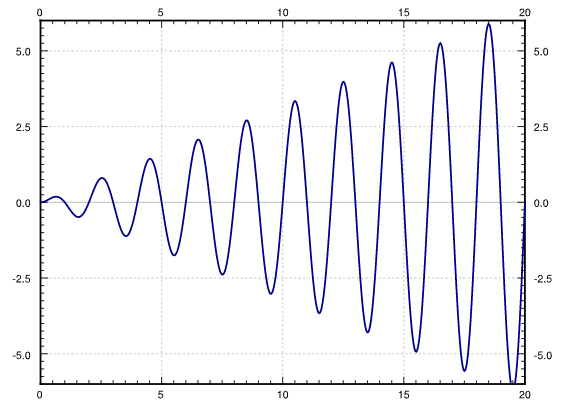
\includegraphics[scale=0.8]{Images/ODEPictures/resonance.png}}

\textbf{Beats}\\
This also occurs where there is no dampening force but where the natural frequency and the driving frequency are different. The particular solution will take the form $x_p=a\cos(\omega t)+b\sin(\omega t)$. This will result the general solution being a sum of waves with different frequencies. This creates a pattern where you have a larger modulating wave comprised of smaller oscillations.\\
\centerline{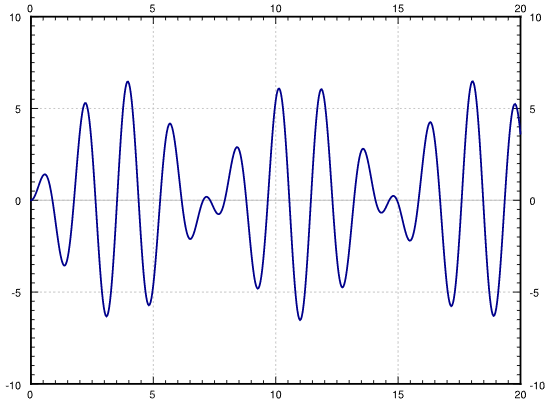
\includegraphics[scale=0.8]{Images/ODEPictures/Beats.png}}

\textbf{Steady State Response}\\
This is the case when there is a dampening force. This means that the complementary solution will experience exponential decay, going away quickly while the particular solution will take the form $x_p=a\cos(\omega t)+b\sin(\omega t)$. In this case, we call the complementary solution the \textit{transient} solution as it goes away fast, leaving the particular solution as what is seen after a long time which we call the \textit{steady state response}. $\lim\limits_{t\to\infty}x(t)=x_p$\\
\centerline{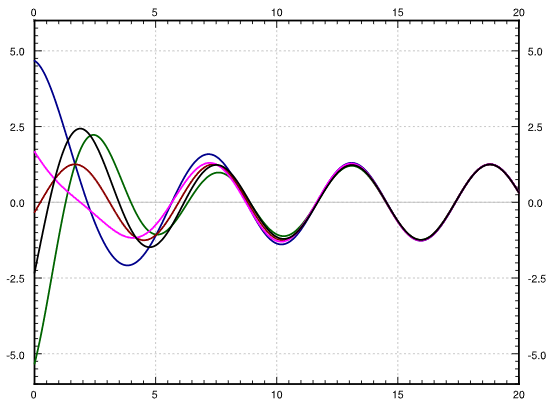
\includegraphics[scale=0.8]{Images/ODEPictures/steadyStateResponse.png}}
Derivation of general form:
\begin{align*}
    &mx''+cx'+kx=F_0\cos(\omega t)\\
    &x_p=a\cos(\omega t)+b\sin(\omega t)\\
    &x_p'=-a\omega\sin(\omega t)+b\omega\cos(\omega t)\\
    &x_p''=-a\omega^2\cos(\omega t)-b\omega^2\sin(\omega t)\\
    &\eqnsystem{-ma\omega^2+bc\omega+ak=F_0\\-mb\omega^2-ac\omega+bk=0}\Ra\matrixx{k-m\omega^2 & c\omega\\-c\omega & k-m\omega^2}\matrixx{a\\b}=\matrixx{F_0\\0}\\
    &\matrixx{k-m\omega^2 & c\omega\\-c\omega & k-m\omega^2}^{-1}=\frac{1}{(k-m\omega^2)^2+(c\omega)^2}\matrixx{k-m\omega^2 & -c\omega\\c\omega & k-m\omega^2}\\
    &\matrixx{a\\b}=\frac{1}{(k-m\omega^2)^2+(c\omega)^2}\matrixx{k-m\omega^2 & -c\omega\\c\omega & k-m\omega^2}\matrixx{F_0\\0}=\frac{F_0}{(k-m\omega^2)^2+(c\omega)^2}\matrixx{k-m\omega^2\\c\omega}\\
    &x_p=\frac{F_0}{(k-m\omega^2)^2+(c\omega)^2}((k-m\omega^2)\cos(\omega t)+c\omega\sin(\omega t))=R\cos(\omega t+\phi)\\
    &R=\sqrt{a^2+b^2}=\frac{F_0}{(k-m\omega^2)^2+(c\omega)^2}\sqrt{(k-m\omega^2)^2+(c\omega)^2}=\frac{F_0}{\sqrt{(k-m\omega^2)^2+(c\omega)^2}}\\
    &\phi=\arctan\brround{\frac{b}{a}}=\arctan\brround{\frac{c\omega}{k-m\omega^2}}\\
    &x_p=\frac{F_0}{\sqrt{(k-m\omega^2)^2+(c\omega)^2}}\cos\brround{\omega t+\phi}
\end{align*}
While this solution cannot achieve pure resonance as in an undamped solution, it can attune a resonance frequency such that the amplitude will approach a maximum. If we consider the amplitude as a function of frequency, we can get the following graph for various values of $m$, $k$, and $c$.\\
\centerline{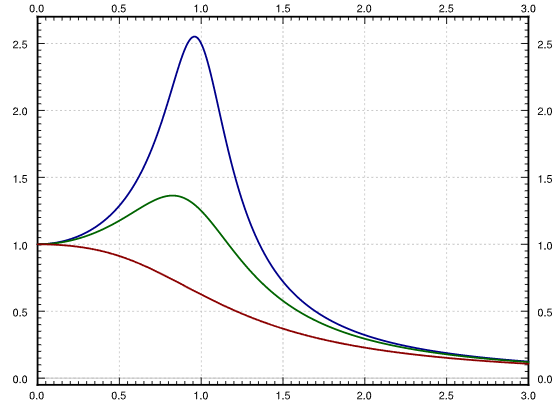
\includegraphics[scale=0.8]{Images/ODEPictures/steadyStateAmplitude.png}}
A frequency of $0$ will give $R=\frac{F_0}{k}$ and a very large frequency will give an amplitude of $R=0$. To find the maximum frequency, we can take the derivative.
\begin{align*}
    &R'(\omega)=\frac{-F_0(2(k-m\omega^2)(-2m\omega)+2c^2\omega)}{2\brround{(k-m\omega^2)^2+(c\omega)^2}^{3/2}}=0\\
    &\omega(-4m(k-m\omega^2))+2c^2)=0\\
    &\omega=0\text{ or,}\\
    &k-m\omega^2=\frac{2c^2}{4m}\Ra k-\frac{2c^2}{4m}=m\omega^2\\
    &\omega=\sqrt{\frac{k}{m}-\frac{c^2}{2m^2}}
\end{align*}
This gives the resonance frequency. If there are no nonzero solutions, we say that the system has no resonance frequency.
\subsubsection{Cauchy-Euler Equation}
The Cauchy-Euler equation is a 2nd order ODE of the form
$$ax^2y''+bxy'+cy=0$$
To solve this equation, we will guess that the solution will be of the form $y=x^r$.\\
This gives $y'=rx^{r-1}$ and $y''=r(r-1)x^{r-2}$\\
So if we plug these into the original equation we get
\begin{align*}
    &ar(r-1)x^r+brx^r+cx^r=0\\
    &x^r(ar^2+(b-a)r+c)=0\\
    &ar^2+(b-a)r+c=0
\end{align*}
giving the characteristic equation.\\
We can solve for $r$ and get 3 cases:\\
Real roots: $(b-a)^2-4ac>0$
\begin{align*}
    &r=\frac{-(b-a)\pm\sqrt{(b-a)^2-4ac}}{2a}\\
    &y(x)=C_1x^{r_1}+C_2x^{r_2}
\end{align*}
Imaginary roots: $(b-a)^2-4ac<0$\\
\begin{align*}
    &r=-\frac{(b-a)}{2a}\pm i\frac{\sqrt{4ac-(b-a)^2}}{2a}=\lambda\pm i\mu\\
    &y(x)=C_1x^{(\lambda+i\mu)x}+C_2x^{(\lambda-i\mu)x}\\
    &y=x^\lambda\brround{C_1x^{i\mu}+C_2x^{-i\mu}}\\
    &y=x^\lambda\brround{C_1e^{i\mu\ln x}+C_2e^{-i\mu\ln x}}\\
    &y=x^\lambda\brround{C_1\cos(\mu\ln x)+C_2\sin(\mu\ln x)}
\end{align*}
Repeated roots: $(b-a)^2-4ac=0$
\begin{align*}
    &r=\frac{a-b}{2a}\\
    &y_1=x^{r}\\
    &y_2=u(x)y_1=u(x)x^r\\
    &y_2'=urx^{r-1}+u'x^r\\
    &y_2''=x^ru''+2u'rx^{r-1}+ur(r-1)x^{r-2}\\
    &ax^{r+2}u''+2arx^{r+1}u'+ar(r-1)x^ru+bx^{r+1}u'+brx^ru+cx^ru=0
\end{align*}
Simplifying we can get that all the $u$ terms cancel out
\begin{align*}
    &\frac{a-b}{2}\brround{\frac{a-b}{2a}-1}+\frac{b(a-b)}{2a}+c\\
    &\frac{a^2-2ab+b^2}{4a}+\frac{-2a^2+2ab}{4a}+\frac{2ab-2b^2}{4a}+\frac{4ac}{4a}\\
    &\frac{-a^2+2ab-b^2+4ac}{4a}=-\frac{(a-b)^2-4ac}{4a}=0
\end{align*}
So our remaining terms are
\begin{align*}
    &ax^{r+2}u''+2arx^{r+1}u'+bx^{r+1}u'=0\\
    &\text{let }v=u'\Ra v'=u''\\
    &ax^{r+2}v'+2arx^{r+1}v+bx^{r+1}v=0\\
    &v'+\frac{2ar+b}{a}\frac{v}{x}=0\\
    &v'+\frac{a-b+b}{a}\frac{v}{x}=0\\
    &v'+\frac{v}{x}=0\\
    &\mu(x)=e^{\int\frac{dx}{x}}\\
    &\mu v'+\mu\frac{v}{x}=xv'+v=\frac{d}{dx}vx=0\\
    &\int\brround{\frac{d}{dx}vx}dx=\int0dx=C\\
    &vx=u'x=C\\
    &\int\frac{du}{u}=\int\frac{dx}{x}\\
    &u(x)=\ln|x|\\
    &y_2=x^r\ln|x|\\
    &y(x)=C_1x^r+C_2x^r\ln|x|
\end{align*}
Note that we can also write a Cauchy-Euler Equation in the form of
$$a(x-\alpha)^2y''+b(x-\alpha)y'+cy=0$$
and our fundamental guess would be of the form $y=(x-\alpha)^r$.\\
Ex:
\begin{align*}
    &x^2y''-xy'+y=0\\
    &y=x^r,\ y'=rx^{r-1},\ y''=r(r-1)x^{r-2}\\
    &r(r-1)-r+1=0\\
    &r^2-2r+1=0\Ra (r-1)^2\Ra r=1\\
    &y=C_1x+C_2x\ln|x|
\end{align*}
Ex2:
\begin{align*}
    &x^2y''-xy'+5y=0\\
    &y=x^r,\ y'=rx^{r-1},\ y''=r(r-1)x^{r-2}\\
    &r(r-1)-r+5=0\Ra r^2-2r+5=0\\
    &r=\frac{2\pm\sqrt{4-20}}{2}=1\pm2i\\
    &y=x(C_1\cos(2\ln|x|)+C_2\sin(2\ln|x|))
\end{align*}
Ex3:
\begin{align*}
    &2x^2y''-xy'+y=x\\
    &y_c=x^r,\ y_c'=rx^r,\ y_c=r(r-1)x^r\\
    &2r(r-1)-r+1=0\Ra 2r^2-3r+1=0\Ra (2r-1)(r-1)=0,\ r=\frac{1}{2},1\\
    &y_c=C_1\sqrt{x}+C_2x\\
    &y_p=ax\ln x\\
    &y_p'=a\ln x+a\\
    &y_p''=\frac{a}{x}\\
    &2ax-ax\ln x-ax+ax\ln x=x\\
    &\Ra a=1\\
    &y=C_1\sqrt{x}+C_2x+x\ln x
\end{align*}